%!LW recipe=beamer + bib
\documentclass[10pt, aspectratio=169, t]{beamer}
\usetheme[
    block=fill,
    progressbar=foot,
    numbering=fraction
]{metropolis}
\usepackage{xspace}
\usepackage{appendixnumberbeamer}
\usepackage{luatexja}
\usepackage[haranoaji, deluxe, expert]{luatexja-preset}
\renewcommand{\kanjifamilydefault}{\gtdefault}
\usepackage{graphicx}
\usepackage{tabularx}
\usepackage{booktabs}
\usepackage{multirow}
\usepackage{qrcode}
\usepackage{tikz}
\usetikzlibrary{arrows.meta, positioning, fit, calc}
\usepackage{luatexja-fontspec}
\usepackage{pgfpages}
%\setbeameroption{show notes on second screen}
\metroset{sectionpage=none}

\usepackage{csquotes}
\usepackage[backend=biber, style=numeric, sorting=none]{biblatex}
\addbibresource{../../paper/sigagi/refs.bib}
\AtEveryBibitem{\clearfield{url}\clearfield{doi}\clearfield{eprint}\clearfield{urlyear}\clearlist{location}\clearfield{pages}}

% Auto-generated by scripts/analyze.py. DO NOT EDIT.
% Reference macros with trailing {} in body text to preserve spacing:
%   e.g. \bestModel{} で ... , \nModels{} 種のモデル

% ==== Experiment scale ====
\newcommand{\nModels}{12}
\newcommand{\nConfigs}{4}
\newcommand{\nItems}{30}
\newcommand{\nCombos}{1440}
\newcommand{\nVendors}{3}
\newcommand{\totalSpend}{\$79.79}

% ==== Bootstrap 95% CI for best combo ====
\newcommand{\bestCIlo}{0.746}
\newcommand{\bestCIhi}{0.903}

% ==== Bootstrap 95% CI for best Single combo ====
\newcommand{\bestSingleModel}{Opus 5}
\newcommand{\bestSingleFtwo}{0.738}
\newcommand{\bestSingleCIlo}{0.645}
\newcommand{\bestSingleCIhi}{0.848}

% ==== Best F2 combo ====
\newcommand{\bestModel}{GPT-5 mini}
\newcommand{\bestConfig}{Multi-run}
\newcommand{\bestFtwo}{0.826}
\newcommand{\bestCost}{\$0.0206}

% ==== Cost spread ====
\newcommand{\cheapestCost}{\$0.0005}
\newcommand{\priciestCost}{\$0.2182}
\newcommand{\costSpread}{415}

% ==== Per-model best-config wins ====
\newcommand{\modelMultiWins}{8}
\newcommand{\modelAdvWins}{0}
\newcommand{\modelSingleWins}{2}
\newcommand{\modelParWins}{2}

% ==== Per-config mean F2 / cost ====
\newcommand{\singleMeanF}{0.536}
\newcommand{\singleMeanCost}{\$0.0196}
\newcommand{\parallelMeanF}{0.514}
\newcommand{\parallelMeanCost}{\$0.0628}
\newcommand{\adversarialMeanF}{0.479}
\newcommand{\adversarialMeanCost}{\$0.0453}
\newcommand{\multiMeanF}{0.602}
\newcommand{\multiMeanCost}{\$0.0939}

% ==== Pareto-dominated models ====
\newcommand{\dominatedModels}{Sonnet 5，GPT-5，Opus 5，Fable 5，GPT-5.6 luna，GPT-5.6 terra，o3，Gemini 3.6 flash，Gemini 3.1 pro-preview}
\newcommand{\dominatedCount}{9}

% ==== Per-repo (language) best (model / config) ====
\newcommand{\bestByFastapi}{GPT-5 mini / Multi-run}
\newcommand{\bestByFastapiF}{0.722}
\newcommand{\bestByValibot}{GPT-5 mini / Multi-run}
\newcommand{\bestByValibotF}{0.777}
\newcommand{\bestByChi}{GPT-5 mini / Multi-run}
\newcommand{\bestByChiF}{0.972}
\newcommand{\bestByPgrust}{GPT-5 mini / Multi-run}
\newcommand{\bestByPgrustF}{0.909}

% ==== Category breakdown ====
\newcommand{\nCategories}{8}
\newcommand{\catWinners}{GPT-5 mini (5 種別)，Haiku 4.5 (3 種別)}
\newcommand{\perfectCats}{other・type-safety・api-misuse・error-handling}
\newcommand{\perfectCount}{4}
\newcommand{\hardestCat}{concurrency}
\newcommand{\hardestBestFtwo}{0.667}
\newcommand{\catNmin}{1}
\newcommand{\catNmax}{15}



\definecolor{slidealert}{HTML}{EB811B}

\makeatletter
\setlength{\metropolis@progressinheadfoot@linewidth}{1pt}
\setbeamertemplate{frametitle}{%
  \nointerlineskip%
  \begin{beamercolorbox}[
      wd=\paperwidth,
      sep=0pt,
      leftskip=\metropolis@frametitle@padding,
      rightskip=\metropolis@frametitle@padding,
    ]{frametitle}
  \metropolis@frametitlestrut@start
  \ifnum\value{section}>0\relax
    \ifnum\value{subsection}=0\relax
      \thesection.\
    \else
      \thesection.\arabic{subsection}\ 
    \fi
  \fi
  \insertframetitle
  \nolinebreak
  \metropolis@frametitlestrut@end%
  \end{beamercolorbox}
}
\makeatother

% Manual break: the auto wrap split the compound 欠陥検出性能 mid-word.
\title{AI コードレビュー・オーケストレーション構成のコスト-欠陥検出性能比較}
\subtitle{第33回汎用人工知能研究会(SIG-AGI)}
\date{2026/08/21}
\author{高原 大明}
\institute{
北陸先端科学技術大学院大学\\
先端科学技術研究科 先端科学技術専攻\\
人間情報学研究領域\\
社会的信号処理・マルチモーダルインタラクション研究室}

\begin{document}
\maketitle

\begin{frame}{Contents}
    \tableofcontents[hideallsubsections]
\end{frame}

\section{背景と課題}

\begin{frame}{構成の優位は，計算量と分離しないと確かめられない}
    汎用人工知能には，\alert{限られた計算資源の下で多様な課題を効率的に解く}能力が要る．\\
    エージェントを何体・何回動かすかという資源配分は，その中心的な設計問題である．

    \vspace{6pt}
    LLM コードレビューの構成比較は\alert{計算量 (コスト) を統制しておらず}\cite{codeagent,guo2024largelanguagemodelbased}，\\
    観測された差が構造由来か計算量由来か切り分けられない．\\
    一般推論では予算を揃えると優位が消える報告があるが\cite{mad,reflexion,wang2024rethinkingboundsllmreasoning}，\\
    コードレビューには\alert{誤りの非対称性}があり，同じ結論が成り立つかは未検証である．

    \vspace{6pt}
    \begin{center}
        \small レビューにおける 2 種類の誤りと，その対処コスト\\[3pt]
        \footnotesize
        \begin{tabular}{@{}lll@{}}
            \toprule
            誤り & 内容 & 対処に要するもの \\
            \midrule
            誤指摘 (FP) & 存在しない欠陥を挙げる & レビュアが却下すれば済む \\
            見逃し (FN) & 実在する欠陥を挙げない & 発見に人手のコードレビュー \\
            \bottomrule
        \end{tabular}
    \end{center}
\end{frame}

\begin{frame}{予算帯によって，最適な構成は入れ替わる}
    \begin{description}
        \item[RQ1] 同等コスト水準で，構成間に欠陥検出率・偽陽性率の差があるか．
        \item[RQ2] 観点別並列の優位は，同コストの Multi-run と比べても残るか．
        \item[RQ3] 欠陥の種別によって有利な構成は異なるか．
    \end{description}

    \vspace{10pt}
    \begin{center}
        \small 本発表の結論：予算帯ごとに最も高い $F_2$ を出した組み合わせ\\[3pt]
        \begin{tabular}{@{}lll@{}}
            \toprule
            項目あたり予算 & 最良の (モデル / 構成) & 含意 \\
            \midrule
            \$0.002 & Haiku 4.5 / Single & 追加呼び出しの費用が支配的 \\
            \$0.01 & \alert{GPT-5 mini / Adversarial} & オーケストレーションが逆転 \\
            \$0.05 以上 & \alert{GPT-5 mini / Multi-run} & 廉価モデルが Opus 5 単体を上回る \\
            \bottomrule
        \end{tabular}
    \end{center}

    \vspace{6pt}
    \nModels{} モデル中 \dominatedCount{} モデルは，全 \nConfigs{} 構成がパレートフロントから脱落した．
\end{frame}

\section{ベンチマーク構築}

\begin{frame}{fix コミットの逆適用で，正解が一意な課題を合成する}
    \begin{center}
    \begin{tikzpicture}[
        node distance=6mm,
        box/.style={draw, rounded corners=2pt, align=center, inner sep=5pt, font=\small},
        arr/.style={-{Stealth[length=5pt]}, thick}
      ]
      \node[box] (fixed) {fix コミット $F$ 適用後\\(正常なコード)};
      \node[box, right=14mm of fixed] (pr) {レビュー対象の差分\\($F^{-1}$ を適用した PR)};
      \node[box, right=14mm of pr] (rev) {LLM レビュアの指摘\\(file, line, 内容)};
      \node[box, below=9mm of rev] (gt) {正解 $=$ $F$ の変更箇所};
      \draw[arr] (fixed) -- node[above, font=\scriptsize] {逆適用} (pr);
      \draw[arr] (pr) -- node[above, font=\scriptsize] {レビュー} (rev);
      \draw[arr] (gt) -- node[right, font=\scriptsize] {\ 突合 ($\pm 2$ 行)} (rev);
    \end{tikzpicture}\\[3pt]
    \scriptsize fix が追加した行を削除した差分を PR として提示し，その見落としを指摘できるかを評価する
    \end{center}

    \vspace{4pt}
    \begin{itemize}
        \item 全リポジトリ・全バグに一律の手続きを適用でき，正解も一意に定まる．
        \item 限界：合成 PR であり，実在した PR ではない．
    \end{itemize}
\end{frame}

\begin{frame}{4 言語 85 件，うち pgrust はカットオフ後だけの統制群}
    \begin{columns}[T]
    \begin{column}{0.42\textwidth}
        \centering
        \small 対象リポジトリと採用件数\\[3pt]
        \footnotesize
        \begin{tabular}{@{}llr@{}}
            \toprule
            リポジトリ & 言語 & 件数 \\
            \midrule
            fastapi & Python & 25 \\
            valibot & TypeScript & 20 \\
            chi & Go & 15 \\
            pgrust & Rust & 25 \\
            \midrule
            \multicolumn{2}{@{}l}{計} & 85 \\
            \bottomrule
        \end{tabular}
    \end{column}
    \begin{column}{0.56\textwidth}
        \begin{itemize}
            \item リポジトリ効果と言語効果を分離するため，\\各リポジトリを単一言語で揃えた．
            \item \textbf{pgrust} は全履歴が対象モデルのカットオフ後 $\rightarrow$ \alert{leakage-free な統制群}．
            \item 境界を 2026-01-01 とし，\\カットオフ前後を共変量として保持 (post 49 / pre 36)．
            \item 分類は Claude 系，検証は異系統 LLM (GPT 系) 17 件で 12 件一致．
        \end{itemize}

        \vspace{4pt}
        \scriptsize 構築：候補 1{,}544 $\rightarrow$ 機械フィルタ 816 $\rightarrow$ LLM 分類 201 $\rightarrow$ 逆適用可 135 $\rightarrow$ 層別抽出 85 件
    \end{column}
    \end{columns}
\end{frame}

\section{実験設計}

\begin{frame}{Multi-run を「構造を持たない計算量増加」の対照群に置く}
    \begin{center}
        \small 比較する 4 構成と，1 件あたりの LLM 呼び出し回数\\[3pt]
        \small
        \begin{tabular}{@{}p{20mm}p{64mm}p{20mm}@{}}
            \toprule
            構成 & 手続き & 呼び出し \\
            \midrule
            Single & 単一レビュアが全観点を担当 & 1 回 \\
            Parallel & 4 観点 (correctness, concurrency, api-misuse, security) を独立実行し和集合 & 4 回 \\
            Adversarial & 指摘生成の後，各指摘に反証プロンプトを 2 回適用し半数以上の支持で採用 & $1 + 2k$ 回 \\
            \alert{Multi-run} & 同一プロンプトを 5 回実行し，2 票以上を採用 & 5 回 \\
            \bottomrule
        \end{tabular}
    \end{center}

    \vspace{4pt}
    \begin{itemize}
        \item システムプロンプトの基底は全構成で共通，出力は \texttt{\{file, line, severity, category, summary\}} の JSON 配列．
        \item \alert{Multi-run は構造を持たない計算量増加}であり，RQ2 の対照群となる．
    \end{itemize}
\end{frame}

\begin{frame}{見逃しの方が対処コストが高いので $F_2$ を主指標に置く}
    \begin{equation*}
        F_\beta = \frac{(1 + \beta^2)\,PR}{\beta^2 P + R}
        \qquad\text{本研究は }\ \alert{\beta = 2}
        \quad\Rightarrow\quad
        F_2 = \frac{5PR}{4P + R}
    \end{equation*}

    \begin{itemize}
        \item $\beta$ は再現率 $R$ を適合率 $P$ の何倍重視するかの重み．\\
            $\beta = 2$ は $\beta^2 = 4$，すなわち\alert{再現率を 4 倍重視}することを意味する．
        \item 誤指摘は却下すれば済むが，見逃したバグの発見には人手レビューが要る．\\
            この非対称性に合わせ，見逃しを減らす側に重みを置いた．
        \item 検出判定：指摘の (file, 行範囲) が正解の変更範囲と重なるかを機械判定 (許容 $\pm 2$ 行)．
        \item 規模：\nVendors{} ベンダ \nModels{} モデル $\times$ \nConfigs{} 構成 $\times$ \nItems{} 件 $=$ \alert{\nCombos{} 実行}，総 API 支出 \totalSpend{}．
    \end{itemize}
\end{frame}

\section{結果}

\begin{frame}{\nModels{} モデル中 \dominatedCount{} モデルは全構成が脱落した}
    \begin{center}
        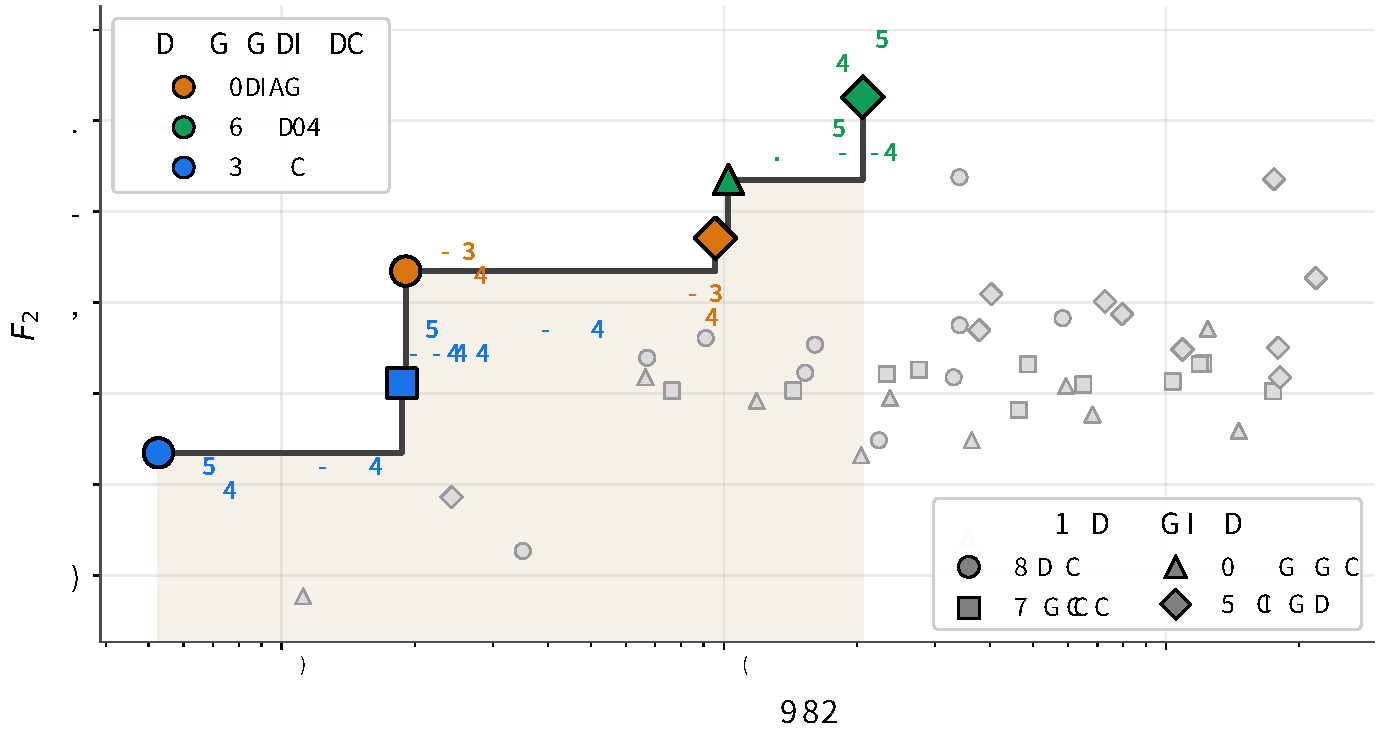
\includegraphics[height=0.74\textheight]{fig/pareto_slide.pdf}\\[2pt]
        \scriptsize 項目あたりコスト (対数軸) と $F_2$ の散布．マーカ形状が構成，フロント上の点のみベンダ色で示す
    \end{center}
\end{frame}

\begin{frame}{再現率の重みを変えても Multi-run が最高}
    \begin{columns}[T]
    \begin{column}{0.44\textwidth}
        \centering
        \small 構成別の平均 $F_\beta$\\[3pt]
        \footnotesize
        \begin{tabular}{@{}lrrrr@{}}
\toprule
Config & $F_{1}$ & $F_{1.5}$ & $F_{2}$ & $F_{3}$ \\
\midrule
Single & 0.619 & 0.563 & 0.536 & 0.514 \\
Parallel & 0.424 & 0.477 & 0.514 & 0.556 \\
Adversarial & 0.572 & 0.508 & 0.479 & 0.456 \\
Multi-run & \textbf{0.665} & \textbf{0.623} & \textbf{0.603} & \textbf{0.585} \\
\bottomrule
\end{tabular}
\\[4pt]
        \scriptsize $\beta$ を 1〜3 に振っても Multi-run が最高
    \end{column}
    \begin{column}{0.54\textwidth}
        \begin{itemize}
            \item 平均 $F_2$ の順位は \alert{Multi-run} $>$ Single $>$ Parallel $>$ Adversarial．
            \item Adversarial：反証で適合率は上がるが，\\\alert{本物のバグまで却下}して再現率が下がる．
            \item Multi-run：2/5 のしきい値が\\適合率と再現率の\alert{双方}を伸ばす．
            \item RQ2 への答え：観点別並列の優位は，\\同コストの計算量増加に対して\alert{残らない}．
        \end{itemize}
    \end{column}
    \end{columns}
\end{frame}

\begin{frame}{\$0.01 を境にオーケストレーションが Single を逆転する}
    \begin{center}
        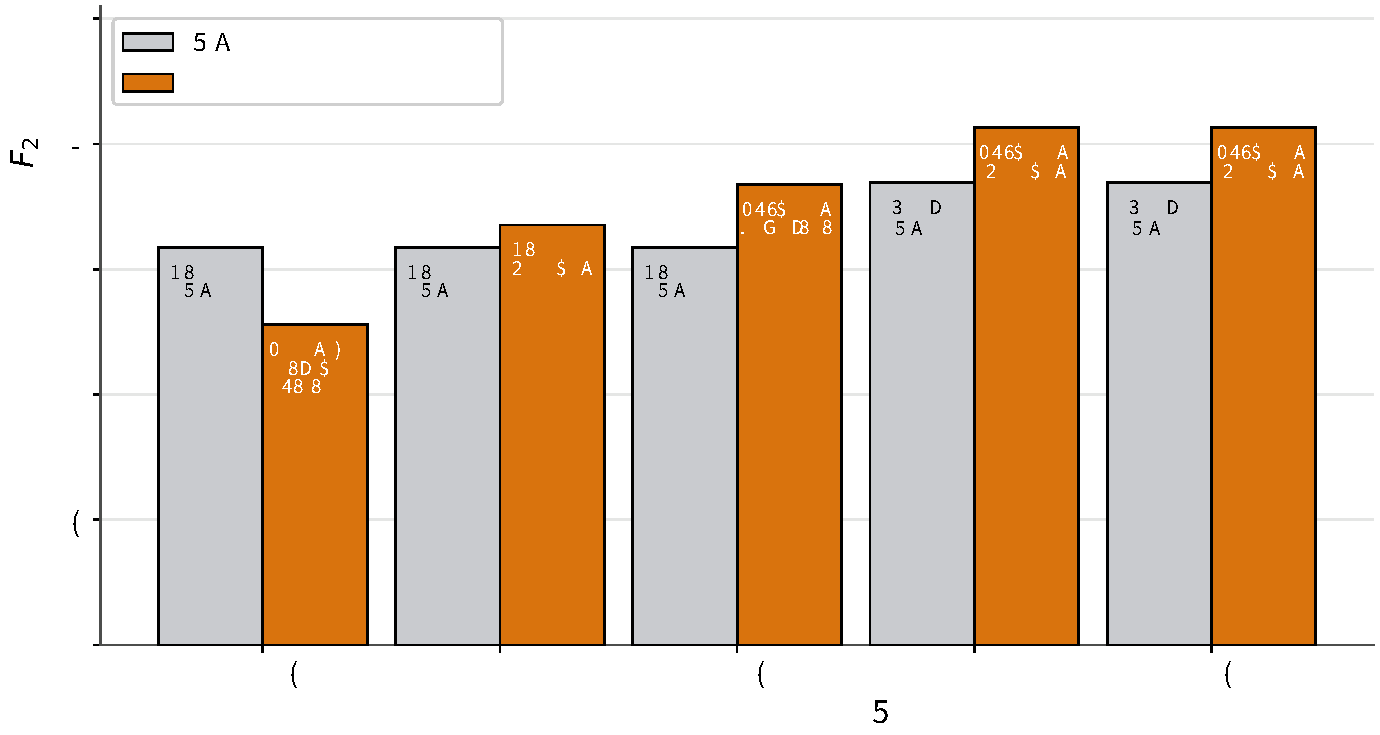
\includegraphics[height=0.70\textheight]{fig/budget_slide.pdf}\\[2pt]
        \scriptsize 予算上限ごとの最高 $F_2$．\$0.05 以上では GPT-5 mini / Multi-run が Opus 5 単体を含む全 Single を上回り，予算を 4 倍にしても天井は上がらない
    \end{center}
\end{frame}

\begin{frame}{バグ種別ごとに最良の (モデル, 構成) は入れ替わる}
    \begin{columns}[T]
    \begin{column}{0.54\textwidth}
        \centering
        \small バグ種別ごとの最高 $F_2$\\[3pt]
        \scriptsize
        \resizebox{\linewidth}{!}{\begin{tabular}{@{}lllr@{}}
\toprule
バグ種別 & 最良 (モデル / 構成) & $F_2$ & N \\
\midrule
logic & GPT-5 mini / Multi-run & 0.779 & 15 \\
type-safety & Haiku 4.5 / Single & 1.000 & 2$^{\dagger}$ \\
error-handling & Haiku 4.5 / Multi-run & 1.000 & 1$^{\dagger}$ \\
concurrency & Haiku 4.5 / Adversarial & 0.667 & 3 \\
api-misuse & GPT-5 mini / Multi-run & 1.000 & 4 \\
security & GPT-5 mini / Adversarial & 0.833 & 1$^{\dagger}$ \\
resource-leak & GPT-5 mini / Multi-run & 0.897 & 2$^{\dagger}$ \\
other & GPT-5 mini / Adversarial & 1.000 & 2$^{\dagger}$ \\
\bottomrule
\end{tabular}
}
    \end{column}
    \begin{column}{0.44\textwidth}
        \begin{itemize}
            \item 最良は種別ごとに異なり，\\\catWinners{} に分かれる．
            \item 最難は \hardestCat{} (最良でも $F_2 = \hardestBestFtwo{}$)．
            \item 言語別では 4 リポとも GPT-5 mini / Multi-run が最良だが，\\達成値は \bestByFastapiF{} (Python) 〜 \bestByChiF{} (Go) と幅がある．
            \item 種別あたり N は \catNmin{}〜\catNmax{} 件と小さく，\alert{予備的示唆}にとどまる．
        \end{itemize}
    \end{column}
    \end{columns}
\end{frame}

\begin{frame}{単一組の有意差は示せない．支えるのは横断的な一貫性}
    \begin{center}
    \begin{tikzpicture}[x=17cm, y=1cm]
      \draw[gray!60] (0.62,0) -- (0.93,0);
      \foreach \v in {0.65, 0.70, 0.75, 0.80, 0.85, 0.90}
        \draw[gray!60] (\v,0) -- (\v,-0.10) node[below, font=\scriptsize, color=black] {\v};

      \fill[gray!18] (0.746,0.55) rectangle (0.848,2.05);

      \draw[very thick, slidealert] (0.746,1.75) -- (0.903,1.75);
      \draw[slidealert, thick] (0.746,1.62) -- (0.746,1.88);
      \draw[slidealert, thick] (0.903,1.62) -- (0.903,1.88);
      \fill[slidealert] (0.826,1.75) circle (2.6pt);
      \node[above, font=\small] at (0.826,1.90) {GPT-5 mini / Multi-run \quad $F_2 = 0.826$};

      \draw[very thick, gray!70] (0.645,0.85) -- (0.848,0.85);
      \draw[gray!70, thick] (0.645,0.72) -- (0.645,0.98);
      \draw[gray!70, thick] (0.848,0.72) -- (0.848,0.98);
      \fill[gray!70] (0.738,0.85) circle (2.6pt);
      \node[below, font=\small] at (0.738,0.70) {Opus 5 / Single \quad $F_2 = 0.738$};
    \end{tikzpicture}\\[2pt]
    \scriptsize 項目 bootstrap による $F_2$ の 95\% 信頼区間．灰色の帯は 2 つの区間が重なる範囲を表す
    \end{center}

    \vspace{2pt}
    \begin{itemize}
        \item $N = \nItems{}$ の本実験では，\alert{単一の組どうしの有意差は主張しない}．
        \item 支えるのは，モデル別集計で \nModels{} モデル中 \modelMultiWins{} が Multi-run 最良という\alert{一貫性}と，$\beta \in \{1, 1.5, 2, 3\}$ で順位が変わらない\alert{指標の頑健性}である．
    \end{itemize}
\end{frame}

\section{まとめ}

\begin{frame}{結果の一般化を妨げる制約}
    \begin{itemize}
        \item \textbf{合成 PR}：逆適用 PR は実在した PR ではなく，レビュー体験の再現性に限界がある．
        \item \textbf{位置一致のみの判定}：(file, line) の重なりで判定しており，\\意味的に等価な指摘を取りこぼしうる．
        \item \textbf{標本サイズ}：$N = \nItems{}$，かつバグ種別で均等化しておらず個別順位の信頼性は低い．
        \item \textbf{反証プロンプトの設計依存}：Adversarial は REFUTED 寄りに設計しており，再現率低下の一因の可能性がある．
        \item \textbf{対象の限定}：商用 API \nModels{} モデル，4 リポジトリ 4 言語に限る．
        \item \textbf{予算統制は事後分析}：予算上限を強制したのではなく，実測コストを予算帯に集計して比較している．
    \end{itemize}
\end{frame}

\begin{frame}{構造を足す前に，同コストの反復を対照群に置くべき}
    \begin{enumerate}
        \item \textbf{構造の効果は，計算量と分離して検証しなければならない．}\\
            役割分担 (Parallel) や反証 (Adversarial) は，\\\alert{同コストの単純な反復集約に対して優位を示さなかった}．
        \item \textbf{最適な構造は資源制約の関数であり，固定して選べない．}\\
            同じ予算で「高性能モデル 1 回」と「廉価モデル 5 回」のどちらが勝つかは，\alert{予算帯で入れ替わった}．
        \item \textbf{タスクを見て構成を切り替えるメタ制御が要る．}\\
            バグ種別によって最良の (モデル, 構成) が入れ替わり，単一の万能構造では届かない．
    \end{enumerate}

    \vspace{6pt}
    コードレビューは正解が機械判定でき，コストが API 課金で正確に測れる．\\
    人手評価に頼らず予算-性能のトレードオフを反復実験できる，\\AGI 研究の実験場として扱える領域である．
\end{frame}

\begin{frame}{まとめ}
    \begin{itemize}
        \item バグ修正コミットの逆適用により，\alert{コストと検出性能を同一軸で比較できる}\\欠陥検出ベンチマークを構築した (4 言語 85 件)．
        \item \nCombos{} 実行の実測から，\\予算帯に依存して最適構成が入れ替わるパレートフロントを提示した．
        \item 構造化された構成 (Parallel, Adversarial) の優位は，同コストの単純な反復集約に対して\alert{残らなかった}．
        \item 今後：意味一致判定器の導入，N の拡大と種別均等化，\\複合構成および動的ルーティングの設計比較．
    \end{itemize}

    \vfill
    \begin{minipage}[b]{0.74\textwidth}
        \scriptsize ベンチマーク・実験ハーネス・全実行記録：\\
        \url{https://github.com/hiroaki222/review-orchestration-bench}
    \end{minipage}\hfill
    \begin{minipage}[b]{0.20\textwidth}
        \raggedleft
        \qrcode[height=2cm, level=M]{https://github.com/hiroaki222/review-orchestration-bench}
    \end{minipage}
\end{frame}

\appendix

\begin{frame}[standout]
    % fin
\end{frame}

\begin{frame}{付録：パレートフロント上の 6 点}
    \begin{center}
        \small コスト-$F_2$ パレートフロントを構成する 6 つの (モデル, 構成)\\[3pt]
        \footnotesize
        \begin{tabular}{llrr}
\toprule
Model & Config & \$/item & $F_2$ \\
\midrule
Gemini 3.5 flash-lite & Single & \$0.0005 & 0.435 \\
Gemini 3.5 flash-lite & Parallel & \$0.0019 & 0.511 \\
Haiku 4.5 & Single & \$0.0019 & 0.635 \\
Haiku 4.5 & Multi-run & \$0.0096 & 0.671 \\
GPT-5 mini & Adversarial & \$0.0102 & 0.735 \\
GPT-5 mini & Multi-run & \$0.0206 & 0.826 \\
\bottomrule
\end{tabular}

    \end{center}

    \vspace{6pt}
    \scriptsize
    \nModels{} モデル $\times$ \nConfigs{} 構成の全 48 セル (適合率・再現率・$F_2$・項目あたりコスト) は論文および公開リポジトリの \texttt{data/experiments/v0/} を参照．
\end{frame}

\begin{frame}{付録：言語別の最良構成}
    \begin{center}
        \small リポジトリ (言語) ごとの最高 $F_2$ とその組み合わせ\\[3pt]
        \footnotesize
        \begin{tabular}{@{}lll@{}}
\toprule
リポジトリ (言語) & 最良 (モデル / 構成) & $F_2$ \\
\midrule
Python (fastapi) & GPT-5 mini / Multi-run & 0.722 \\
TypeScript (valibot) & GPT-5 mini / Multi-run & 0.777 \\
Go (chi) & GPT-5 mini / Multi-run & 0.972 \\
Rust (pgrust) & GPT-5 mini / Multi-run & 0.909 \\
\bottomrule
\end{tabular}

    \end{center}

    \vspace{6pt}
    \begin{itemize}
        \item 4 リポジトリすべてで GPT-5 mini / Multi-run が最良だった．
        \item 達成 $F_2$ の幅は，言語・ドメインが検出難度を左右することを示す．
    \end{itemize}
\end{frame}

\begin{frame}{付録：コストの内訳}
    \begin{itemize}
        \item 項目あたりコストは最安 \cheapestCost{} から最高 \priciestCost{} まで \costSpread{} 倍の広がりを持つが，$F_2$ はコストに単調ではない．
        \item 構成別の平均コスト：Single \singleMeanCost{}，Parallel \parallelMeanCost{}，Adversarial \adversarialMeanCost{}，Multi-run \multiMeanCost{}．
        \item 総 API 支出 \totalSpend{}．全 API 呼び出しの記録 (\texttt{runs/*/ledger.jsonl}) を公開しており，第三者によるコスト再計算が可能である．
    \end{itemize}
\end{frame}

\begin{frame}[allowframebreaks]{参考文献}
    \printbibliography[heading=none]
\end{frame}

\end{document}
